\chapter{METODOLOGI}

% Ubah konten-konten berikut sesuai dengan isi dari metodologi

\section{Tools Yang Akan Digunakan}

Sistem ini dibuat oleh laptop penulis yang menggunakan \emph{operating system} Arch Linux. Prosesornya sendiri menggunakan Intel Core i5
8265U dan RAM 12 GB. \emph{Graphic Card}-nya adalah NVIDIA GeForce MX 250 2GB. Untuk menggunakan Unreal Engine 5, penulis menggunakan PC
dengan sistem operasi Ubuntu 20.04 dan \emph{Graphic Card} NVIDIA GeFoce GTX 1070 TI. Penulis melakukan remote desktop dengan menggunakan aplikasi
NoMachine.

\subsection{\emph{Metamask}}
\emph{Metamask} adalah \emph{crypto walle} yang biasanya digunakan untuk keperluan development. Crypto wallet ini
akan sangat membantu dalam proses pengembangan. Terdapat banyak fitur-fitur seperti multi-account yang mempermudah proses pengembangan.

\subsection{Remix IDE}
Remix IDE merupakan IDE yang memudahkan kita untuk proses development, deployment, dan membuat smart contract di Ethereum.

\subsection{Ethereum}
Ethereum adalah \emph{blockchain opensource} dengan fitur smart contract. Fitur smart contract inilah yang akan digunakan untuk
melakukan sharing data metadata audio.

\subsection{\emph{Solidity}}
Solidity adalah adalah bahasa tingkat tinggi berbasis objek untuk mengimplementasikan
\emph{smart contract}. Solidity ini dijalankan didalam Ethereum Virtual Machine (EVM).
Kontrak di Solidity mirip dengan class dalam bahasa object-oriented.  Secara umum, Solidity untuk Smart Contract dibuat dengan mengirimkan
Ether ke Smart Contract dan mengirim Ether dari Smart Contract menuju address penerima Ether tersebut.

\subsection{\emph{Ganache}}
\emph{Ganache} berguna untuk membuat ethereum blockchain di local network. Tool ini akan digunakan untuk
keperluan development di local sebelum dideploy di testnet.

\subsection{InterPlanetary File System (IPFS )}
Protokol dan peer to
peer network untuk distribusi konten yang cepat, terdistribusi
dan mudah disatukan yang kompatibel untuk semua tipe data
seperti gambar, stream video, database terdistribusi.

\subsection{\emph{web3.storage}}
web3.storage adalah serangkaian API dan layanan yang memudahkan pengembang dan pengguna lain untuk berinteraksi
dengan data dengan cara yang tidak terikat dengan tempat penyimpanan data sebenarnya secara fisik. Service ini menggunakan data terdesentralisasi dan protokol
seperti IPFS, Filecoin, dan UCAN yang memungkinkan arsitektur aplikasi dan alur kerja yang dapat diverifikasi, berpusat pada data dan pengguna.

\section{Desain Arsitektur}
Proses ini memberikan perincian pada sistem yang akan dibuat. Berdasarkan dari latar
belakang masalah dan tujuan dari tugas akhir ini, didapatkan beberapa fungsi yang akan
diimplementasikan pada sistem dan keseluruhan flow sistem.

\subsection{Arsitektur Sistem}

\begin{figure} [ht] \centering
  % Nama dari file gambar yang diinputkan
  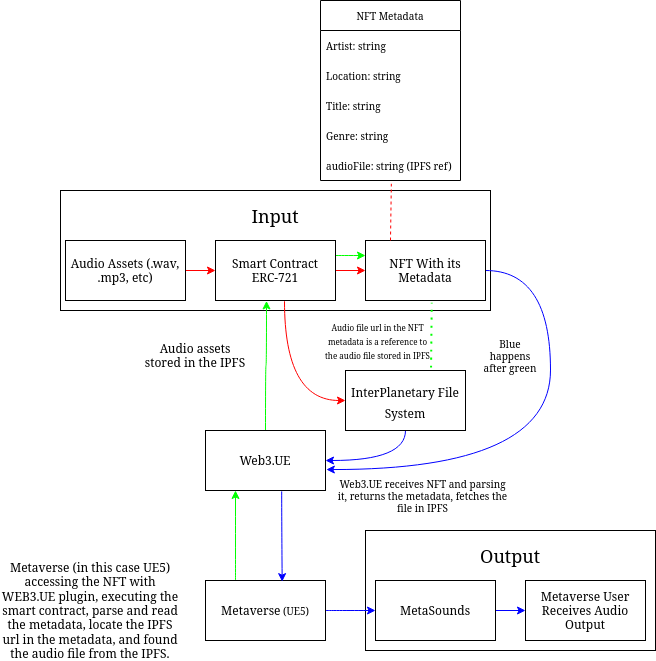
\includegraphics[scale=0.65]{gambar/architecture.png}
  % Keterangan gambar yang diinputkan
  \caption{Diagram Arsitektur Sistem}
  % Label referensi dari gambar yang diinputkan
  \label{fig:Architecture}
\end{figure}

\emph{Smart contract} pada arsitektur berguna untuk melakukan operasi-operasi \emph{blockchain} seperti
memberikan NFT yang berisi metadata dari audio yang sudah disimpan di \emph{blockchain} sebelumnya.
Untuk file dari audio itu sendiri direferensikan oleh metadata pada NFT tersebut dan akan diambil dari
IPFS menggunakan web3.storage. Metaverse disini diimplementasikan menggunakan Unreal Engine 5 dan menggunakan API
\emph{blockchain} untuk mengeksekusi smart contract. File audio akan diolah oleh metasound dan user akan menerima output audio tersebut.
Untuk deskripsi dari metadata tersebut adalah berupa file JSON dan berikut ini merupakan \emph{interface}-nya

% Contoh input potongan kode dari file
\lstinputlisting[
  language=Python,
  caption={Format data audio.},
  label={lst:formatdataaudio}
]{kode/audioData.json}
Proses perancangan dari arsiktektur sistem yang meliputi IPFS, server, dan blockchain.

\subsection{Proses \emph{generate} NFT dari audio}

Untuk melakukan generate NFT diperlukan proses yang dinamakan Token minting.
Crypto minting adalah sebuah proses komputasi untuk memvalidasi informasi, membuat blok baru dan merekam informasi tersebut ke dalam \emph{blockchain}.
Dalam proses crypto minting biasanya membutuhkan algoritma konsensus Proof-of-Stake.

\begin{figure} [ht] \centering
  % Nama dari file gambar yang diinputkan
  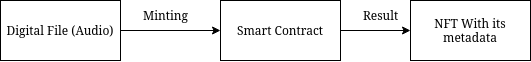
\includegraphics[scale=0.55]{gambar/mintingtoken.png}
  % Keterangan gambar yang diinputkan
  \caption{Diagram Token Minting}
  % Label referensi dari gambar yang diinputkan
  \label{fig:mintingtoken}
\end{figure}

Proof-of-Stake sendiri adalah konsensus yang membantu proses minting seperti bagaimana blok dibuat dan bagaimana data ditambahkan ke blok. Cara kerja crypto minting yaitu koin dicetak (mint) melalui staking di bawah proses Proof-of-Stake. Berbeda halnya dengan Proof-of-Work, Proof-of-Stake tidak memiliki miner. Sebagai gantinya, PoS menggunakan validator. Validator berperan untuk mengamati, juga bertanggung jawab untuk melakukan validasi transaksi dan bekerja untuk menghasilkan blok baru.
Minting adalah proses yang cukup mudah dan terdesentralisasi. Kemudahan dalam proses  minting ini memungkinkan siapa saja untuk membuat token baru tanpa mengharuskan otoritas pusat untuk melakukannya.
Selain itu, ekosistem crypto juga menyediakan berbagai macam token yang diciptakan dengan proses minting, termasuk token aset kripto dan non-fungible token (NFT). Kedua jenis token tersebut tentunya dapat dibuat di berbagai ekosistem blockchain.

\emph{Listing} diatas merupakan \emph{interface} dari metadata yang ditampung di NFT. Semua nilai dari data JSON tersebut
memiliki tipe data yang adalah \emph{string}.

\subsection{\emph{Flow} sistem}
\begin{figure} [ht] \centering
  % Nama dari file gambar yang diinputkan
  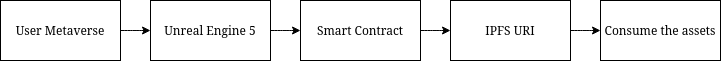
\includegraphics[scale=0.55]{gambar/userinteractionmetaverse.png}
  % Keterangan gambar yang diinputkan
  \caption{Flow interaksi user dengan metaverse}
  % Label referensi dari gambar yang diinputkan
  \label{fig:userinteractionmetaverse}
\end{figure}
\begin{figure} [ht] \centering
  % Nama dari file gambar yang diinputkan
  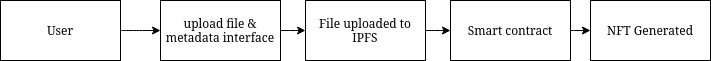
\includegraphics[scale=0.55]{gambar/userinteractionupload.png}
  % Keterangan gambar yang diinputkan
  \caption{Proses yang terjadi saat upload file untuk minting}
  % Label referensi dari gambar yang diinputkan
  \label{fig:userinteractionupload}
\end{figure}

\section{Implementasi}

Pembuatan implementasi dari fitur dari aplikasi yang sudah ditentukan melalui tahap
sebelumnya. Tahap ini dilakukan sampai selesai untuk masuk pada tahap validasi. Alokasi
waktu yang ditentukan menyesuaikan dengan pembuatan fitur yang dikerjakan. Pembuatan
implementasi diperkirakan kurang lebih dua bulan. Implementasi ini termasuk baik pembuatan mini-metaverse
menggunakan \emph{Unreal Engine 5} sebagai sarana untuk melakukan evaluasi dan testing agar keseluruhan sistem dapat terintegrasi.

\begin{figure} [ht] \centering
  % Nama dari file gambar yang diinputkan
  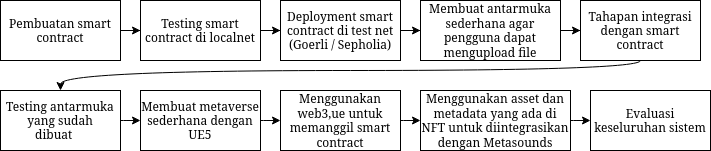
\includegraphics[scale=0.60]{gambar/methodologydiagram.png}
  % Keterangan gambar yang diinputkan
  \caption{Diagram Implementasi}
  % Label referensi dari gambar yang diinputkan
  \label{fig:diagramimplementasi}
\end{figure}

\subsection{Pembuatan \emph{Smart Contract}}
\emph{Smart Contract} diperlukan untuk membuat perjanjian dengan
berbagai kondisi agar pada \emph{blokchain} bisa mengatur sendiri tanpa
adanya pihak ketika, disini dibuat beberapa kondisi pada
smart contract dalam bentuk kode. Pembuatan smart contract dapat mengacu pada dokumentasi resmi maupun eksternal.
Namun perlu dilakukan modifikasi untuk menyesuaikan dengan desain sistem yang digunakan pada penelitian
ini.

\subsection{Proses pembuatan antarmuka untuk mengunggah file audio}
Setelah \emph{Smart Contract} dibuat, maka akan dibuat tambahan antarmuka untuk dapat mengunggah file, dan membuat NFT dari file tersebut.
File yang dibuat akan disimpan di IPFS. NFT yang di\emph{generate} akan menyimpan hash IPFS atau CID yang apabila diakses maka akan ditemukan
file text dengan format \emph{JSON}. File JSON ini akan menyimpan kumpulan \emph{key value}. Salah satu dari \emph{value} ini adalah hash dari source file sound
yang disimpan di IPFS.

\subsection{Pembuatan metaverse sederhana menggunakan Unreal Engine 5}
Pembuatan metaverse ini ditujukan agar dapat menguji dan mengevaluasi apakah \emph{smart contract} yang dibuat pada langkah sebelumnya sudah benar.
Fitur yang menjadi fokus utama adalah fitur sound dari \emph{plugin metasound}. Namun semakin banyak fitur yang dibuat maka semakin bagus hasilnya karena
diusahakan dapat menjadi universal, tidak hanya musik namun juga bisa untuk \emph{sound effect} dan lain sebagainya.

\subsection{Integrasi metaverse dengan sistem blockchain}
\emph{ABI} yang didapatkan dari kompilasi \emph{smart contract} akan digunakan untuk melakukan integrasi dengan Unreal Engine 5.
Setelah itu, akan dilakukan evaluasi dengan cara \emph{Trial and Error} dan melakukan testing untuk kecepatan transaksi, dikarenakan
tiap blockchain dapat berbeda kecepatan transaksinya.

\section{Jadwal Pelaksanaan}

% Ubah tabel berikut sesuai dengan isi dari rencana kerja
\newcommand{\w}{}
\newcommand{\G}{\cellcolor{gray}}
\begin{table}[h!]
  \captionof{table}{Tabel Jadwal Pelaksanaan}
  \label{tbl:timeline}
  \begin{tabular}{|p{3.5cm}|c|c|c|c|c|c|c|c|c|c|c|c|c|c|c|c|}

    \hline
    \multirow{2}{*}{Kegiatan} & \multicolumn{16}{|c|}{Minggu}                                                                       \\
    \cline{2-17}              &
    1                         & 2                             & 3  & 4  & 5  & 6  & 7  & 8  & 9  & 10 & 11 & 12 & 13 & 14 & 15 & 16 \\
    \hline

    % Gunakan \G untuk mengisi sel dan \w untuk mengosongkan sel
    Desain Sistem             &
    \G                        & \G                            & \G & \G & \w & \w & \w & \w & \w & \w & \w & \w & \w & \w & \w & \w \\
    \hline

    Implementasi              &
    \w                        & \w                            & \G & \G & \G & \G & \G & \G & \G & \G & \G & \G & \w & \w & \w & \w \\
    \hline

    Testing                   &
    \w                        & \w                            & \w & \w & \w & \w & \w & \w & \w & \w & \G & \G & \G & \w & \w & \w \\
    \hline

    Evaluasi penelitian       &
    \w                        & \w                            & \w & \w & \w & \w & \w & \w & \w & \w & \w & \w & \G & \G & \G & \G \\
    \hline

    Penyusunan buku           &
    \w                        & \w                            & \w & \w & \w & \G & \G & \G & \G & \G & \G & \G & \G & \G & \G & \G \\
    \hline
  \end{tabular}
\end{table}
